\section{\method: A Framework for Creating Users Profiles }

This section describes \method, the framework proposed to identify semantic
profiles for a set of targeted users from Twitter. As previously described,
the users profiles are a set of weighted preferences, representing a semantic
topic frequently discussed in their posts $D$.  Figure~\ref{frameworkFig}
illustrates the framework.  Steps one to four, i.e.,text
preprocessing, data modelling and extraction of latent factors, do not differ
from what has been done in the literature so far. The main contribution of the
framework is steps five to nine, where semantic sub-topics are merged into
semantic groups and then used to describe user preferences. Finally, these
user preferences are used to generate users semantic profiles.

The text preprocessing phase follows the traditional steps of text
preprocessing in information retrieval, which includes the removal of special
characters, stop-words, plural and genre
markers, and the conversion of verbs to infinitive.  After preprocessing, the
data modelling phase creates a matrix, given as input to a matrix
factorization method.

The data has three dimensions to be considered as part of the matrix: users,
terms and posts. Our final goal is to identify the topics most discussed by
the users in a given domain. Hence, one intuitive representation would be a
matrix of \textit{users} x \textit{terms}, once topics appear from
correlations between terms, and we want to associate topics with users.

However, the set of terms that represent a user will probably refer to more than one topic. As a post is usually made of one sentence expressing the user's opinion or preference in a specific matter, sets of posts will represent sets of topics. For this reason, data is represented as a matrix of \textit{posts} $\times$ \textit{terms}, making the correlation between different topics simpler to identify.
The term associated with each position in the matrix is represented using the term frequency (TF), which showed better results than a TF~X~IDF representation. 
%Although tests with TF~X~IDF were performed, tests with TF were performed better, as the definition of topic is a \emph{frequently mentioned} concept in a set of posts.

After these initial steps, the resulting matrix is used to identify latent factors or semantic sub-topics (representing relations between different terms) using a Non-negative Matrix Factorization (NMF) methods, which generates semantic topics that will be associated with user preferences. From the set of user preferences, users profiles are generated. These two steps are detailed in the next sections. 


\subsection{Identifying latent factors}
\label{primaryFactors}

As discussed in Section~\ref{sec:related}, 
many works in the literature have dealt with the problem of identifying latent factors. Here we work with NMF because it does not assume that latent factors compose
a space of independent variables. Further, NMF provides a more intuitive modelling of documents through these factors, defining each document
as a sum of positive components. We can briefly describe NMF as follows. Given an input matrix $A \in \mathbb{R}^{m \times n}$,
where each line represents a post and each column represents a term, and an integer  $k$ $<$ $min\{m, n\}$, representing the number of desired latent factors, NMF finds two non-negative matrices $W$ $\in$ $\mathbb{R}^{m \times k}$ and $H$ $\in$ $\mathbb{R}^{n \times k} $, where $A$ $\approx$ $W H^T$.

Defining $k$ for NMF is not simple, since it is widely
believed that NMF is a non-convex problem with a unique solution, and only local minima can be found \cite{lin2007convergence}. Here we propose a heuristic for finding $k$ based on the variability analysis of the post collection, as the objective of this phase is to identify as many distinct relevant topics as possible.

\begin{figure}[!t]
\centering
	\epsfig{file=figures/framework.eps,width= 3.2in,height=2.25in}
%	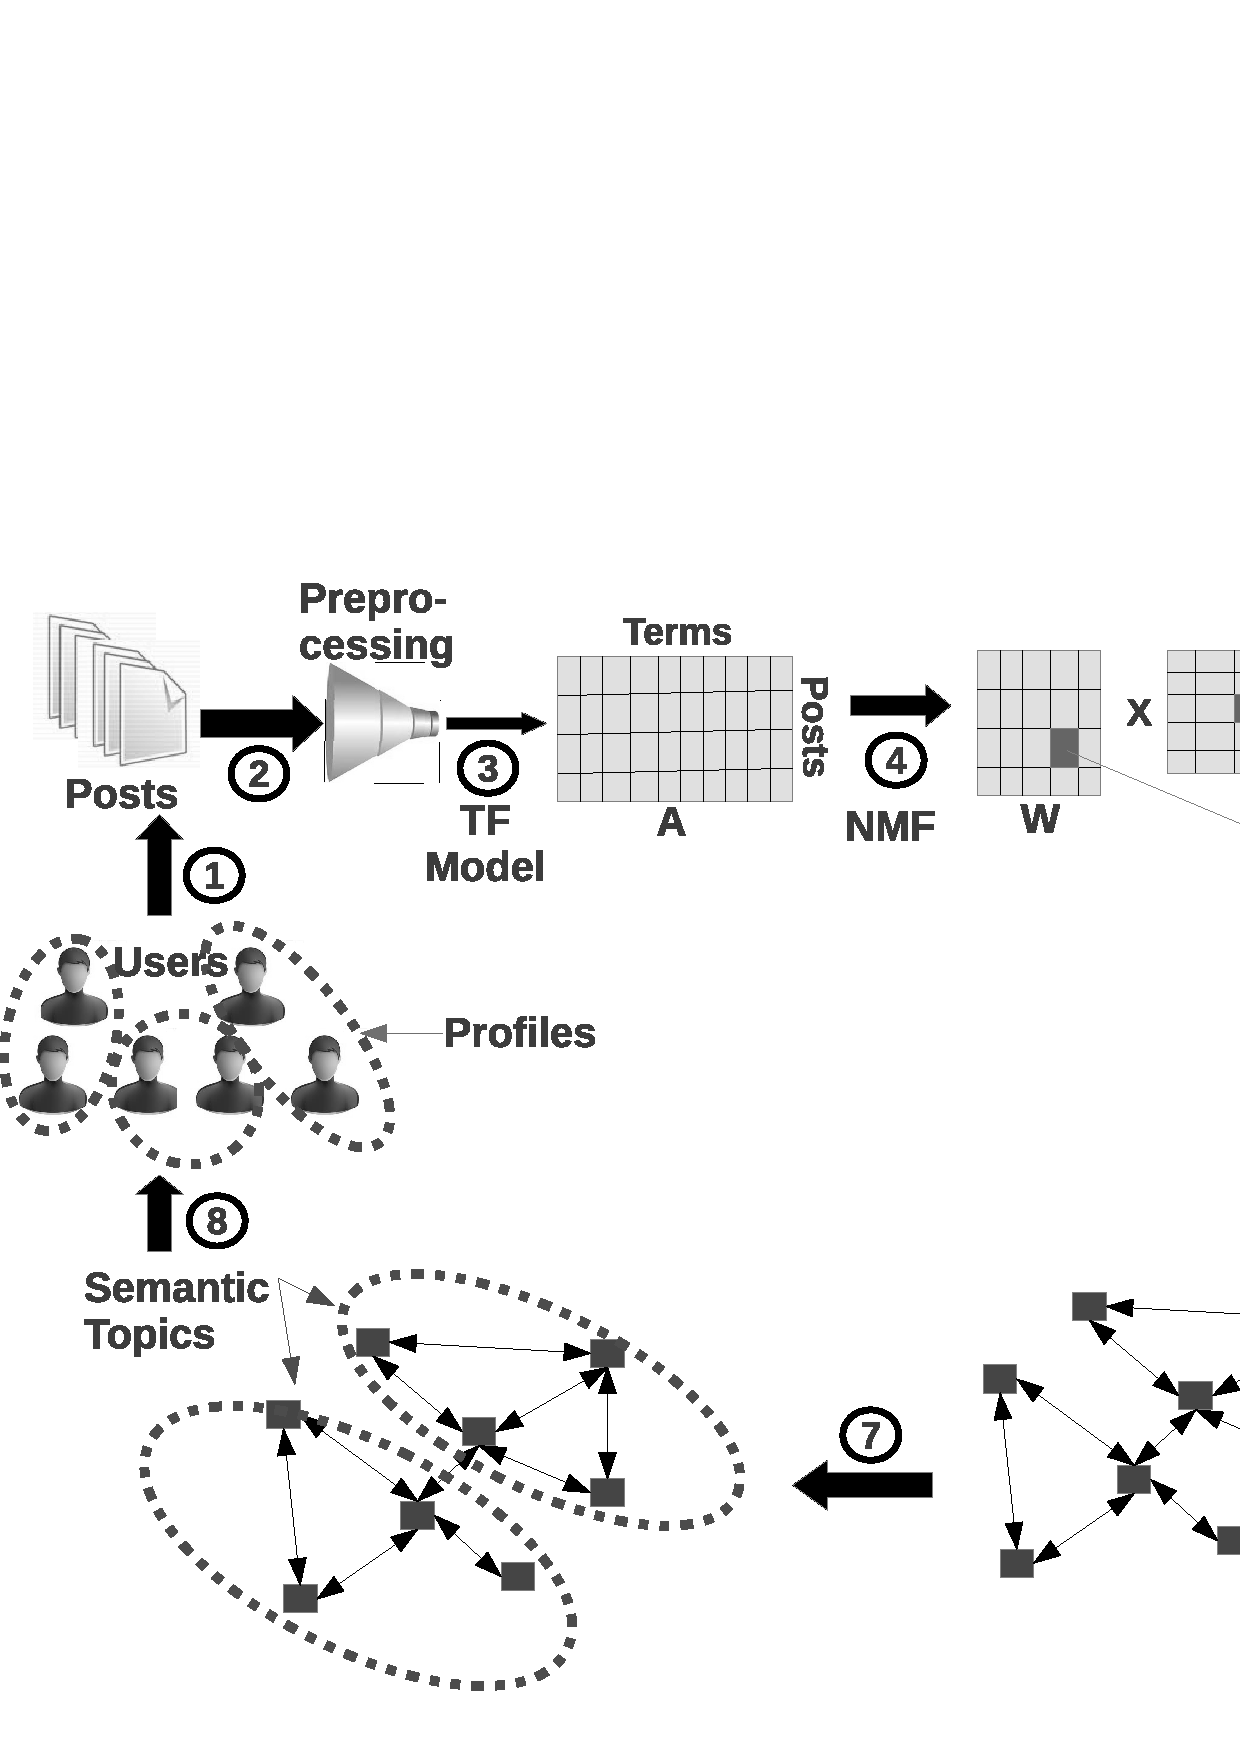
\includegraphics[width= 3.4in,height=2.45in]{figures/framework.pdf}
\vspace{-0.25cm}
\caption{\method: a framework for user semantic profile identification}
\label{frameworkFig}
\vspace{-0.25cm}
\end{figure}


% WMJ: premissa muito forte.
%We assume that the x\% most representative topics would define around x\% of the observed variability on each
%collection and vice-versa. 

We assume that the dimensions of highest variability define the most representative topics on each collection.
Thus, by knowing the number $k$ of topics necessary to provide x\% variability is enough to identify the number of most representative topics. In this sense, we run a Principal Component Analysis (PCA) method 
to estimate $k$. The rationale behind this choice is that the PCA is well-known for returning an ordered set of linearly
independent components that represent the dimensions of most variability on the data. According to the theory of Principal Component Analysis (PCA) \cite{johnson2002applied}, the total population variance (tpv) can be described as $\sum_{i=1}^{k} \lambda_{i}$, 
%\[
%\mbox{Total Populational Variance} = \sum_{i=1}^{k} \lambda_{i}
%\]
where $\lambda_{i}$ is the $i^{th}$ eigenvector of the co-variance matrix associated with the input matrix of posts $\times$ terms $A$ \cite{johnson2002applied}. 

The number $k$ of eigenvectors is chosen based on the desired $tpv$, or
equivalently to the percentage of desired representativeness. Hence, the framework replaces $k$ by a more intuitive parameter, which is the x\% most representative topics. 

%Again, it is important to emphasize that it is a heuristic, since NMF does not guarantee to find the $k$ dimensions of most variability. However, since matrix $W$ and $H$ found by NMF are non-orthonormal bases that minimize a $k\mbox{-}rank$ approximation to the original matrix $A$, in general its local minima solutions provide good approximations. However, bounds on the quality of NMF solutions is an open question in the literature \cite{berry2007algorithms}.

\subsection{Finding Semantic Topics}
\label{sec:merge}

We have already discussed that matrix factorization methods produce semantic
sub-topics, but they are not able to guarantee that the latent factors found
represent \textbf{distinct}, \textbf{representative} and \textbf{cohesive}
semantic topics. These three properties are important to show the topics are
as independent and disjunctive as possible.  According to these properties,
the semantic topic identification problem can be defined as: identify the
minimum number of semantic topics that represent, with high intern cohesion
and low fragmentation the most representative topics in a set of posts $D$.
Note that we are not interested in identifying all topics, but the most
representative subset.

The main objective of \method is to find topics with these three properties, which is a real challenge. Representativeness refers to the frequency of
the topics in D. However, it cannot be directly measured once different
vocabularies might refer to the same topic. These different vocabularies have
a direct impact on cohesion. Cohesion is defined as the capacity of a topic
being associated with a single subject. Finally, the topics have to be the
least fragmented as possible. This is necessary because topics are actually a
hierarchy of subtopics. For instance, when we talk about sports, we can talk
about football or tennis. In general, the existing techniques are able to
define each subtopic as a distinct topic, which generates a fragmented set of
topics about the same subject. This is one of the main differences from our
method to the others: identify non-fragmented semantic topics.

In order to merge semantic sub-topics, we first assume latent factors are modelled by a stochastic process, and that there is a
probability of reaching a factor $f'$ when leaving a factor $f$. Hence, we first represent the users, posts and terms as a tripartite graph, and transform it into a transition graph between different latent factors. We then perform a random walk between latent factors on this graph, and merge factors with high probabilities of mutually reaching each other.


\subsubsection{Creating a tripartite graph}

The NMF output matrices describe the relations between the latent factors found and the input terms and posts. The output $m \times k$ matrix $W$ represents the $m$ input posts through $k$ latent
factors. Each value $W_{ij}$ greater than zero defines both a directed edge
from post $p_i$ to latent factor $f_j$ and an edge in the opposite direction
from $f_j$ to $p_i$. Similarly, matrix $H$ of $n \times k$ dimensions
describes each term through $k$ factors, and each cell $H_{ij}$ greater than
zero defines a relation between a term and a latent factor.\looseness=-1

%\begin{figure}[!ht]
%\centering
%	\subfigure[]{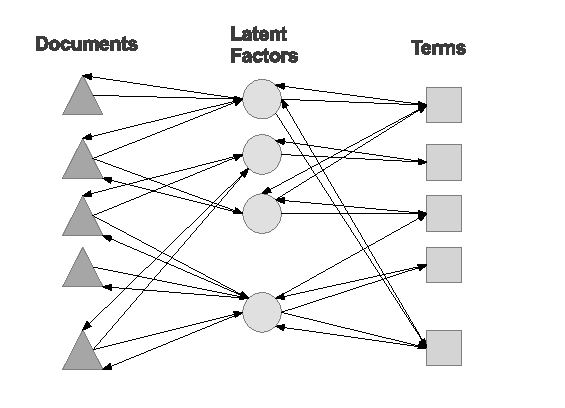
\epsfig{file=figures/tripartiteGraph.eps,width= 2.3in,height=1.45in}} \label{tripartiteGraph}
%	\hfill
%	\subfigure[]{}
%\epsfig{file=figures/tripartiteSemanticGraph.eps,width= 2.3in,height=1.45in}
%\vspace{-0.25cm}
%\caption{Example of a Tripartite Graph}\label{tripartiteGraph}
%\end{figure}

Based on this relation, we build a weighted directed tripartite graph $G_t$ with three types of nodes $T$, $F$ and $D$,
representing the terms, latent factors and posts, respectively.
%, as illustrated in Figure~\ref{tripartiteGraph}.
The intuition behind this graph is that a term can be associated with more than one latent factor (e.g., the term \textit{depression} might be present in the topic about health and politics with different meanings) as a post can talk about one or more latent factors (e.g., the same post can talk about sports and food ``Watching the football at Albanos while eating the best pesto spaghetti ever \#goPSG"). 
Each edge weight represents the intensity of the relationship between
two nodes, and the graph weights are given by the values of $W$ and $H$. As the values of the output matrices of
NMF are always positive, we used the normalized values of $W_{ij}$ and $H_{ij}$ as edge weights. Edges leaving a
term or post towards a latent factor, $W_{ij}$ or $H_{ij}$, are normalized by the sum of the values in the $i^{th}$
line of $W$ or $H$, making the sum of all leaving probabilities equals to $1$. Analogously, for edges leaving from
latent factors to terms/posts, we normalize their values by the sum of the values of the $j^{th}$ column.


\subsubsection{Building the Topic Transition Graph}

From the tripartite graph $G_t$, we want to convert it into a new graph $G$ describing only relationships between
latent factors in $F$. 
As the edge weights in $G$ are normalized, each weight can be interpreted
as a probability of leaving one node and reaching directly a different one. Following this rationale, each latent factor
$f_i \in F$ has also an indirect probability of reaching another factor $f_j \in F$ through terms and posts. We want to
transform these indirect links into direct relations between factors. 
Having a graph that represents only latent factors, we can then calculate the probabilities of a random walker leaving a  latent factor $f_i$ and reaching a latent factor $f_j$.
In order to do that, we transform this two-step probabilistic
paths into a single edge by using Equation~\ref{transitionEquation}. Note that we join these probabilities by summing up their results, but other kinds of combinations could be tested.

\begin{scriptsize}
\begin{equation} \small
P(f_i \!\rightarrow \!f_j)\! = \!\!\sum_{k \in T^{f_i}}\!\!\! P( t_k|f_i) \times P( f_j|t_k)  + \!\sum_{k \in D^{f_i}}\!\!\! P(d_k|f_i) \times P (f_j|d_k) \\
\label{transitionEquation}
\end{equation}
\end{scriptsize}
%P(f_i, f_j) = \sum_{k \in T^{f_i}} P(f_i, t_k) \times P(t_k, f_j) + \sum_{k \in D^{f_i}} P(f_i, d_k) \times P(d_k, f_j)

\noindent where $T^{f_i}$ and $D^{f_i}$ are the sets of terms and posts with an input edge $f_i$. In Equation~\ref{transitionEquation},
the first sum represents all indirect paths from $f_i$ to $f_j$ passing through the terms, while the second comprises the indirect paths through documents.

The resulting graph $G$ is represented by a stochastic transition matrix $M$,
i.e., where the sum of each row in $M$ is equal to 1. As we are concerned
with semantic relations among latent factors, and that not semantically
correlated topics may share a subset of terms, it is important to distinguish
effective relations from noisy ones. A noisy relation is defined as an edge in
$G_i$ with transition probability smaller than the random transition
probability in a graph of the same size. Noisy relations are identified and
removed from $G$ by setting to zero their corresponding cells in matrix $M$. In
order to ensure that $M$ remains stochastic, we re-normalize each of its rows.
Further, in order to ensure that the random walking process conducted in the
next step converges to a unique solution, we make $G$ irreducible (all of its nodes are mutually reachable)
and aperiodic (there is no integer $S > 1$ that divides the length of every cycle of the graph). \looseness=-1

%[TODO: falar que em geral por construçao a matriz atende a estas
%exigencias....] Here we adopted the same solution used by Pagerank
%\cite{CITAR}, defining a $damp factor$ for random transitions in the $G_1$.

\begin{algorithm}[!t]
    \begin{algorithmic}[1]
    \begin{small}
    \Function{joinTopics}{$k$, $M$, $\alpha$}
 

        \While{ $k > 1$}
           \State \label{point1} $P_{min}$ = getMinTransitionProbability(M)
            \State \label{point2} $M'$ = modifyTransitionMatrix(M)
            \State \label{point3} candidatePairList = getImpact($M'$, $k$, $\alpha$)
            \State \label{point4}candidatePair $\gets$ getBestImpactPair(candidateList)
            \While{impact (candidatePair) $>$ 0}

                \State updateTransitionMatrix($M$, candidatePair)
                \State $k --$
                \State candidate $\gets$ getBestImpactPair(candidateList)
            \EndWhile                
        \EndWhile
        \State $\Return M$        
    \EndFunction

    \Function{getImpact}{$M_t$, $k$, $\alpha$}
        \For{ $i = 1 \to k$ }
            \For{ $j = i+1 \to k$ }
                \State $M_t'$ = mergeTopics($M_t$, i, j)
                \State $\Delta_{Coh}$ = cohesionDifference($M_t$,$M_t'$)
                \State $\Delta_{Uni}$ = uniquenessDifference($M_t$,$M_t'$)
                \State impact(i,j) = $\alpha \times \Delta_{Coh}$ + (1.0 - $\alpha$)$ \times \Delta_{Un}$
            \EndFor
        \EndFor
        \State $\Return$ impact
    \EndFunction
    \end{small}
    \end{algorithmic}
\caption{\textbf{Merging latent factors}}
%\vspace{-0.1cm}
\label{joinAlgorithm}
\end{algorithm}

\subsubsection{Merging Topics}


Having the topic transition graph, the next step of our method is to merge semantic
sub-topics.  The idea is to merge topic pairs with a high mutual probability
of reaching each other while the gains regarding \textit{uniqueness} surpass
the losses regarding \textit{cohesion}, as described in
Algorithm~\ref{joinAlgorithm}.  The algorithm receives as inputs the number of latent
factors identified in Section~\ref{primaryFactors} (represented by
$k$), the transition matrix $M$ generated in the previous step and the
linear weight $\alpha$ that determines the relative relevance of
\textit{uniqueness} gains and \textit{cohesion} losses, once they are
contradictory goals, as explained below. 

The algorithm is iterative, and at each iteration a minimum transition
probability $P_{min}$ is defined between all pairs of topics $a$, $b$ in $M$
as the mean probability of a random walker go from $a$ to $b$ (without using
self-loops) times the probability of the random walker go from $a$ to any
topic chosen at random (line \ref{point1}).  Next, as the graph $G$
represented by $M$ is not usually a clique, line \ref{point2} calculates the
probabilities of nodes not directly connected reach each other, generating
$M'$. As $M$ is irreducible, this information is obtained by exponentiating
$M$ $d$ times ($M^d$), where $d$ is the diameter of $G$.\looseness=-1


Next, in line~\ref{point3}, the function \textit{getImpact} calculates,
for each pair of topics, the impact that merging them will produce in $M'$
w.r.t. \textit{fragmentation} and \textit{cohesion}.  $\Delta_{Cohesion}$ is
given by the difference between the minimum transition probability among distinct
topics in $G$ and the random transition probability in a clique with $N$
distinct topics over the random transition probability.  The higher the minimum
transition probabilities observed among topics in $G$ when compared to a
random walk in a clique, the more cohesive $G$ is.  $\Delta_{Unicity}$, in
turn, is defined as the difference between the mutual transition probability
between two distinct topics $i$ and $j$ selected to be merged, and the minimum
transition probability among topics $G$ over the minimum transition probability.
In this case, the higher the mutual transition probability, the higher the
gains w.r.t. uniqueness in merging $i$ and $j$.  

Equations
\ref{cohesionDefinition} and \ref{unicityDefinition} define the
$\Delta_{Cohesion}$ and $\Delta_{Unicity}$, respectively.
$\overline{reach(G)}$ denotes the minimum transition probability among all pairs
of distinct topics in $G$; $N$ refers to the number of distinct topics of $G$
and $reach_{j,i}(G)$ denotes the transition probability between topics $i$ and
$j$ of $G$. Tests using the average and maximum transition probability for $\overline{reach(G)}$ were also tested, but the values of minimum transition probability presented the best results. \looseness=-1
\begin{small}
\begin{equation}
\label{cohesionDefinition}
	\Delta_{Cohesion} = \frac{\overline{reach(G)} - \frac{1}{N}}{\frac{1}{N}}
\end{equation}
 
\begin{equation}
\label{unicityDefinition}
	\Delta_{Unicity} = \frac{ (\frac{reach_{,i,j}(G) + reach_{j,i}(G)}{2}) - \overline{reach(G)} }{\overline{reach(G)}}
\end{equation}
\end{small}
%%%%%%%%%%%%%%%%%%%%%%%%%%%%%%%%%%%%%%%%%%%%%%%%%%


The impact is defined by the linear combination of uniqueness gains and
cohesion losses weighted by $\alpha$.  If the highest impact of a pair of
topics caused in $M$ is positive, the pair will be merged and $M$ updated by
replacing the two merged pairs with a single new topic and updating their the
transition probabilities of their in- and out-edges. Next, a new topic with
high impact in $M$ is selected, and this process goes on until there are no
remaining topics with probability greater then $P_{min}$, or the number of
resulting topics reaches one. \looseness=-1

%The next step of the algorithm is to run the function $selectedPairs$ by defining the probability  $P_{am}(f_i, f_j)$ of mutual reach between pairs of factors $f_i, f_j \mid i \neq i$, as defined in Equation~\ref{mutualReach}. In Equation~\ref{mutualReach}, $size(f_i)$ returns the number of topics already merged to topic $f_i$, and gives priority to merging smaller topics.
%Having done that, we sort the pairs according to $v$ \gi{o que eh v?}, and select all pairs with probability greater than $P_{min}$ to be merged.

%\begin{equation} \small
%P_{am}(f_i, f_j) = \frac{1}{max(size(f_i), size(f_j))} \times \frac{P(f_i \rightarrow f_j) + P(f_j \rightarrow f_i)}{2}
%\label{mutualReach}
%\end{equation}


At the end of this process, the original latent factors are grouped. As users
generate posts, the relations between users and semantic topics may
be determined indirectly through the posts he/she created.

\subsection{Creating User Profiles}

%The previous sections have described the process for identifying semantic topics from user posts.  
This section shows how posts and users are mapped to semantic topics.  
Algorithm~\ref{joinAlgorithm} outputs a matrix $M$ of
posts per semantic topics, where each cell shows the probability $P_{ij}$ of a
given post $i$ belong to a topic $j$.  Initially we set to 0 all the
probabilities in $M$ that are lower than the random probability of a post
belong to a topic.  From the modified $M$ we extract the probability that a user
$k$ in $U$ talks about a semantic topic given his/her posts according to
Eq.~\ref{eq:fase3}.  In Eq.~\ref{eq:fase3} $P_{k,i}$ represents the uniform
probability of a user posting $i$.  Note that, in this process, a post can be
associated with zero (in case all its probabilities of belonging to a topic
are below random), one or more than one topic.

\begin{equation}
\label{eq:fase3}
\sum_{i,j \in M,  k \in U} {P_{i,j} \times P_{k,i}}
\end{equation}

After this process, we end up with a new matrix $M_u$ of users per topics ($k$ x $j$), which has the probability of each user talking about a topic.
Given this matrix, we can extract general preferences (topics) of the group of users or those more specific to subgroups of users. Here we are interested in the users general preferences, but the method can be easily adapted to work with specific ones by, for instances, clustering the users. 

The general users preferences can be the generated, for example, by calculating the mean or median of the probabilities of all users talk about a topic. By ranking the users' preferences according to any of these simple metrics, we obtain the most popular preferences describing the set of users.
%We could stop the process here, but our intention is to characterize groups of users. Such characterization may be refined through clustering, for instance running the expectation-maximization algorithm \cite{moon1996expectation} to find groups of users.
